\chapter{弦、重力、コンパクト化、T双対性}

\lectureoverview{点粒子は事実上任意の滑らかな幾何学の上を矛盾なく運動できるが、量子弦はそうはいかない。弦の無限に多くの零点振動が、次第に短いスケールで標的空間を探り、それらの振動が回復されるにつれて有効幾何学が変化する。この過程が固定点を持つことを要請すると、\(R_{\mu\nu}=0\)、すなわち真空アインシュタイン方程式が得られる。次にこの整合性条件からコンパクト化へと移る。円はカルツァ--クライン運動量状態と弦の巻き付き状態の両方を与え、それらを交換することは半径\(R\)の円を半径\(\alpha'/R\)の円と同一視する。}

\section{選別原理としての整合性}

答えるべき問いは二つある。なぜ弦理論に重力が現れるのか、そしてなぜ弦理論は点粒子力学よりもはるかに許容的でないのか。これらは実は一つの問いである。背景幾何学が許容されるのは、弦がその上を伝播する際に、我々が弦をどれほど細かく分解するかに任意に依存することを保たずに済む場合だけである。

まず制御問題から始める。滑らかな曲面上に拘束された点粒子である。古典的にはそれは測地線、すなわち直線の内在的類似物に従う。運動を多くの短い線分で近似し、差分方程式を書き、次に線分の長さをゼロに近づけることができる。結果は、よく定義された連続極限を持つ常微分方程式である。

量子力学が変えるのは歴史の和であり、結論ではない。一つの古典的経路を選ぶ代わりに、曲面上の経路にわたって振幅を和する。時間は再び小さなステップに分割でき、その極限は曲がった配置空間上のSchr\"odinger方程式によって等価に記述される。滑らかな曲面に対しては、極限は確定した伝播関数とスペクトルに落ち着く。

\begin{figure}[H]
  \centering
  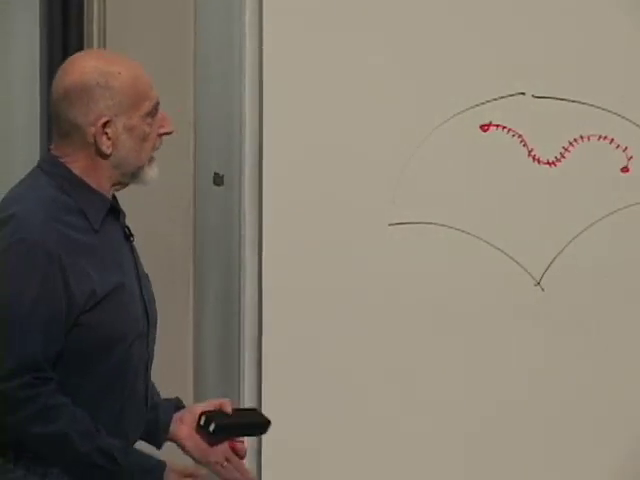
\includegraphics[width=0.72\textwidth]{lecture_09_figure_01.png}
  \caption{曲面上の滑らかな経路と、時間分割された量子和から得られるぎざぎざの経路。どちらも標的曲面に内在したままである。}
  \lectureframe{00:05:10}
  \label{fig:l09-particle-paths}
\end{figure}

\begin{classroomqa}
\audiencequestion{経路積分において、すべての経路は曲面の内部にとどまることが要求されるのですか。\lecturetimestamp{00:05:39}}
\lecturerresponse{はい。曲面は粒子の配置空間であり、粒子が近道を通ることのできるより大きな部屋に埋め込まれたシートではない。すべての中間点は曲面に属し、すべての長さと作用はその内在的計量で計算される。}
\end{classroomqa}

弦に対する対応する問いはより難しい。弦は重心位置だけでは指定されない。弦は無限の振動子の塔を担うので、分解能を上げることはより多くの力学的自由度を認めることを意味する。理論が整合的であるのは、その塔が回復されるにつれて観測量がある極限に近づく場合だけである。

\section{球面上の点粒子}

球面は最も単純な曲がった試験幾何学である。その半径を\(R\)とし、まず質量\(m\)の粒子をその上に置く。大円に沿った運動に対して、
\begin{equation}
  E=\frac{1}{2}mv^2=\frac{p^2}{2m},
  \qquad
  L=pR.
  \label{eq:l09-particle-energy}
\end{equation}
したがって、
\begin{equation}
  E=\frac{L^2}{2mR^2}
   =\frac{L^2}{2I},
  \qquad
  I=mR^2.
  \label{eq:l09-rotor-energy}
\end{equation}
半径は慣性モーメントを通じて入る。角運動量を量子化すると、おなじみの剛体回転子スペクトルが得られ、何も紫外カットオフに依存しない。

\begin{figure}[H]
  \centering
  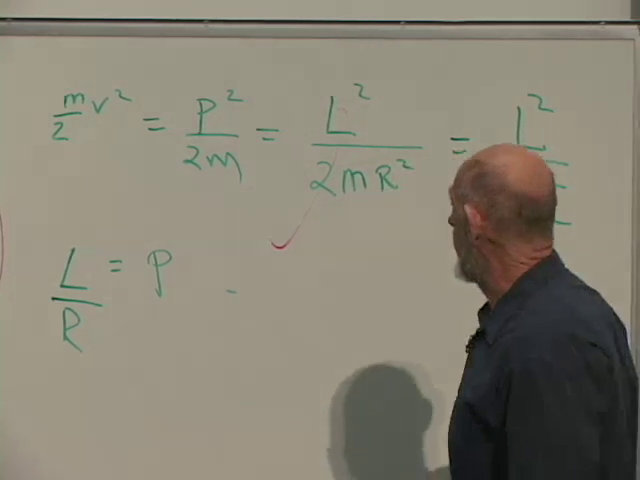
\includegraphics[width=0.74\textwidth]{lecture_09_figure_02.png}
  \caption{点粒子の制御計算：
  \(p^2/(2m)=L^2/(2mR^2)=L^2/(2I)\)。}
  \lectureframe{00:11:25}
  \label{fig:l09-sphere-rotor}
\end{figure}

この平穏な例は重要である。曲率それ自体は問題ではない。問題は、曲率が弦の内部量子的広がりと結合するときに現れる。

\section{真空の弦は点状ではない}

開弦の一つの横座標を考え、その重心を差し引く。ここで用いる振動子展開は模式的なものである：
\begin{equation}
  X(\sigma)-X_{\mathrm{cm}}
  \sim
  \sum_{n=1}^{\infty}
  \frac{a_n+a_n^\dagger}{\sqrt n}\cos(n\sigma).
  \label{eq:l09-mode-expansion}
\end{equation}
本質的な要素は、余弦モード、振動子演算子、そして因子\(1/\sqrt n\)である。正確な規格化は大きさの議論では役割を果たさない。
\editorialnote{正確な展開には、規約に依存する\(\alpha'\)の因子、数値定数、および振動子記法の選択が含まれる。式\eqref{eq:l09-mode-expansion}は、板書での導出と同様に、紫外推定に必要な依存性のみを保持している。}

\begin{figure}[H]
  \centering
  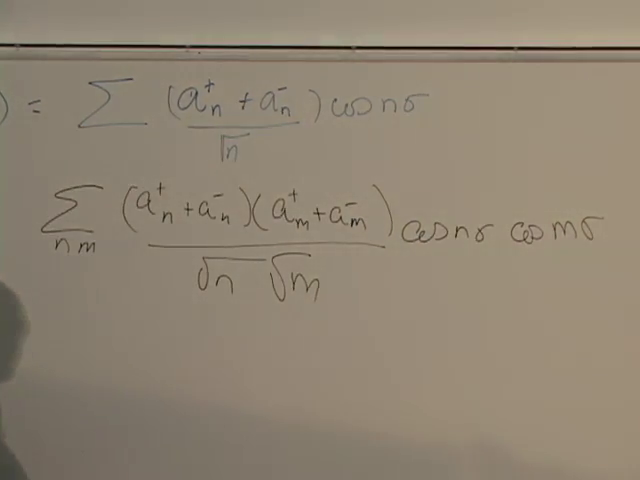
\includegraphics[width=0.78\textwidth]{lecture_09_figure_03.png}
  \caption{構造的な振動子展開と、それを二乗して得られる二重和。}
  \lectureframe{00:15:20}
  \label{fig:l09-string-modes}
\end{figure}

振動子真空における重心からの距離の二乗は
\begin{align}
  \expect{\bigl(X(\sigma)-X_{\mathrm{cm}}\bigr)^2}_0
  &\sim
  \sum_{n,m\geq1}
  \frac{\cos(n\sigma)\cos(m\sigma)}{\sqrt{nm}}\notag\\
  &\qquad\times
  \bra{0}(a_n+a_n^\dagger)\notag\\
  &\hspace{6em}\times(a_m+a_m^\dagger)\ket{0}.
  \label{eq:l09-size-double-sum}
\end{align}
ほとんどの項は消える。二つの消滅演算子はケットを消し、二つの生成演算子はブラに直交する状態を残し、生成演算子の後に消滅演算子が続く場合もこの順序では真空期待値がゼロである。生き残る縮約は
\begin{equation}
  \bra{0}a_n a_m^\dagger\ket{0}=\delta_{nm}.
  \label{eq:l09-vacuum-contraction}
\end{equation}

\begin{figure}[H]
  \centering
  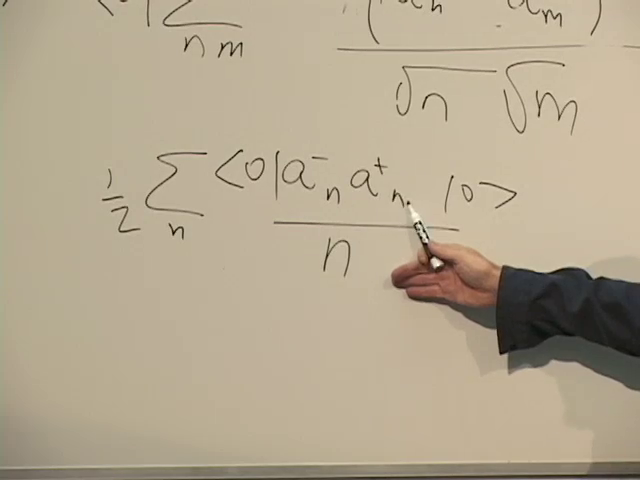
\includegraphics[width=0.74\textwidth]{lecture_09_figure_04.png}
  \caption{生き残った真空の縮約は、二重振動子和を単一の和に崩壊させる。}
  \lectureframe{00:20:10}
  \label{fig:l09-vacuum-contraction}
\end{figure}

したがって
\begin{equation}
  \expect{\bigl(X(\sigma)-X_{\mathrm{cm}}\bigr)^2}_0
  \sim
  \sum_{n=1}^{\infty}\frac{\cos^2(n\sigma)}{n}.
  \label{eq:l09-size-single-sum}
\end{equation}
弦に沿った一般の点では、あるいは\(\sigma\)について平均した後では、
\(\cos^2(n\sigma)\)はおおよそ\(1/2\)に寄与する。モードのカットオフ
\(N\)を導入すると、
\begin{equation}
  \expect{\bigl(X-X_{\mathrm{cm}}\bigr)^2}_{0,N}
  \sim
  \frac{1}{2}\sum_{n=1}^{N}\frac{1}{n}
  =\frac{1}{2}\log N+O(1).
  \label{eq:l09-logarithmic-size}
\end{equation}

\begin{figure}[H]
  \centering
  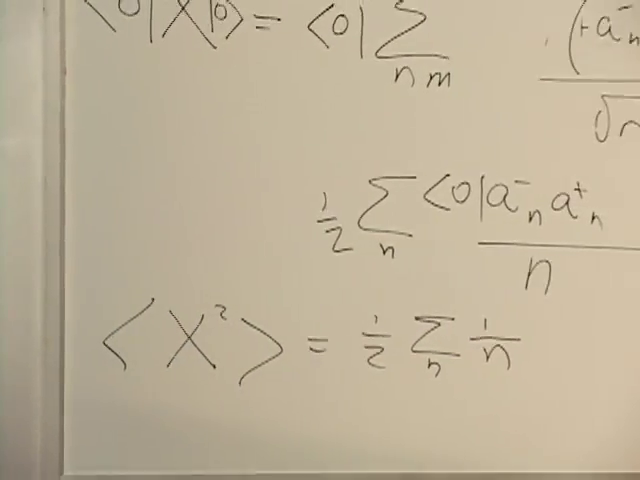
\includegraphics[width=0.72\textwidth]{lecture_09_figure_05.png}
  \caption{黒板は、基底状態の広がりを支配する調和和に到達する。}
  \lectureframe{00:22:05}
  \label{fig:l09-harmonic-size}
\end{figure}

たとえば最初の25個のモードだけを残すと、有限のファジーな対象が得られるが、それはまだ連続的な弦ではない。カットオフを取り除くと、平均二乗広がりは対数的に増大する。この結論は、平坦空間の弦理論が無矛盾でないことの証明と誤読されるべきではない。平坦空間では、重心運動と振動子運動が分離し、物理的振幅における微妙な相殺が期待される局所性を保つ。増大する大きさは警告である。曲率は、その警告が破綻になるかどうかを教えてくれる。

\section{内部の広がりが幾何学を変えるとき}

弦を球の北極の近くに置く。すべての振動子を切ると、それはちょうど調べた点粒子のように振る舞う。より高いモードを許すと、弦はキャップ上に広がった揺らぐもつれとなる。その中心は依然として球の周りを移動しうるが、回転エネルギーに入る慣性モーメントを持つ対象は今や拡がっている。

球の中心と極を通る軸に対して、
\begin{equation}
  I=\int r_\perp^2\,dm,
  \label{eq:l09-extended-inertia}
\end{equation}
ここで\(r_\perp\)は弦の要素からその軸までの垂直距離である。軌道の赤道上の点は最大の関連するてこの腕を持つ。軸に向かって垂れ下がる弦の部分はより少なく寄与する。全質量を固定すると、これは有効慣性モーメントを下げる：
\begin{equation}
  I_{\mathrm{eff}}<mR^2.
  \label{eq:l09-inertia-reduction}
\end{equation}
したがって回転エネルギーは、より小さな球上の点物体のもののように見える：
\begin{equation}
  E_{\mathrm{rot}}
  =\frac{L^2}{2I_{\mathrm{eff}}}
  \equiv \frac{L^2}{2mR_{\mathrm{eff}}^2},
  \qquad R_{\mathrm{eff}}<R.
  \label{eq:l09-effective-radius}
\end{equation}

\begin{classroomqa}
\audiencequestion{弦がより大きな領域に広がっているのなら、なぜ慣性モーメントはゼロに向かうべきなのか。\lecturetimestamp{00:33:23}}
\lecturerresponse{この記述は、逐次的な粗視化の下での有効記述についてのものであり、生の拡がった分布が直ちにゼロの慣性を持つという主張ではない。最初のモードのバンドは、点を、より小さな球上に住んでいるかのように動くファジーな塊に変える。次のバンドは、そのような各塊の内部構造を分解し、同じ繰り込みを繰り返す。この比較を反復すると、有効半径は内側へ駆動される。}
\end{classroomqa}

\begin{figure}[H]
  \centering
  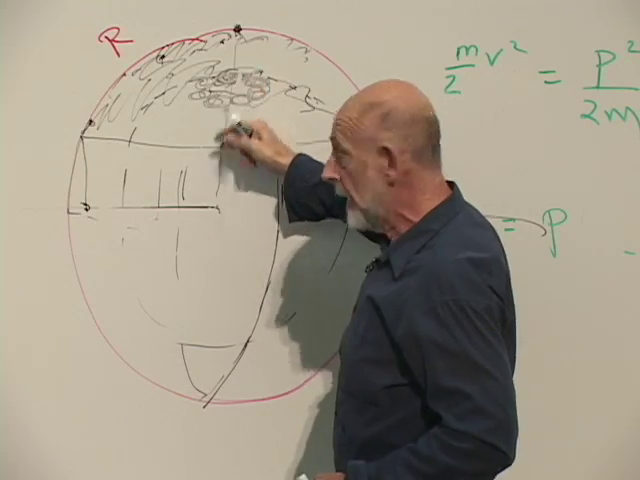
\includegraphics[width=0.72\textwidth]{lecture_09_figure_06.png}
  \medskip

  \begin{adjustbox}{max width=\linewidth}
  \begin{tikzpicture}[x=1cm,y=1cm,>=Latex]
    \draw[thick] (0,0) circle (2.15);
    \draw[dashed] (0,-2.55) -- (0,2.55);
    \draw[blue!65!black,thick]
      (-0.22,2.05)
      .. controls (-1.22,1.75) and (-1.52,1.08) .. (-1.06,0.44)
      .. controls (-0.55,-0.10) and (0.35,0.02) .. (1.10,0.68)
      .. controls (1.48,1.12) and (1.16,1.80) .. (0.20,2.05);
    \draw[red!70!black,dashed] (0,0) circle (1.25);
    \draw[->] (2.70,1.55) -- (4.05,1.55);
    \node[align=center] at (3.37,1.98) {add shorter\\modes};
    \draw[thick] (6.15,0) circle (1.25);
    \draw[dashed] (6.15,-1.65) -- (6.15,1.65);
    \draw[blue!65!black,thick]
      (6.00,1.18)
      .. controls (5.42,0.88) and (5.46,0.25) .. (6.02,-0.06)
      .. controls (6.46,-0.28) and (6.90,0.45) .. (6.28,1.18);
    \node at (0,-3.00) {sphere of radius \(R\)};
    \node at (6.15,-2.05) {effective radius \(R_{\mathrm{eff}}\)};
  \end{tikzpicture}
  \end{adjustbox}
  \caption{黒板上の北極の弦と、有効半径の議論の明快な再構成。破線の内側の円は有効幾何学であり、球の内部の第二の物理的な殻ではない。}
  \lectureframe{00:35:15}
  \label{fig:l09-shrinking-sphere}
\end{figure}

これは繰り込み群の主張である。有限のカットオフは弦を有限の内部分解能を持つ塊にする。カットオフを上げると、その塊の力学が変わる。正に曲がった球上では、追加される各モードの殻が、長距離運動から推測される背景をより小さくする。結果が決して安定しないなら、その背景上にカットオフに依存しない弦理論は存在しない。

\section{計量は固定点に到達しなければならない}

ここで球を一般的な標的空間の計量
\(g_{\mu\nu}(x)\)に置き換える。振動子モードの薄い対数的な殻を積分に入れると、その計量は局所的な対称二階テンソルだけ変化する。変化は平坦空間で消えなければならず、計量の二階導関数から始まらなければならない。主要次数では、共変性によりリッチテンソルが関連する候補として残る：
\begin{equation}
  \frac{\partial g_{\mu\nu}}{\partial\log\Lambda}
  =-C\,R_{\mu\nu}+\cdots ,
  \qquad C>0
  \label{eq:l09-ricci-flow}
\end{equation}
幾何学的議論で用いられた粗視化の方向において。すると正の曲率は、要求されるように球を内側へ駆動する。
\editorialnote{規格化と符号は、繰り込みパラメータが紫外へ向かって増大するか赤外へ向かって増大するかに依存する。従来の世界面の記法では、主要な計量ベータ関数は\(\beta^g_{\mu\nu}=\alpha'R_{\mu\nu}+\cdots\)である。ここで用いられる不変な言明は、カットオフ独立性がベータ関数、したがってこの次数では\(R_{\mu\nu}\)が消えることを要求するというものである。}

\begin{figure}[H]
  \centering
  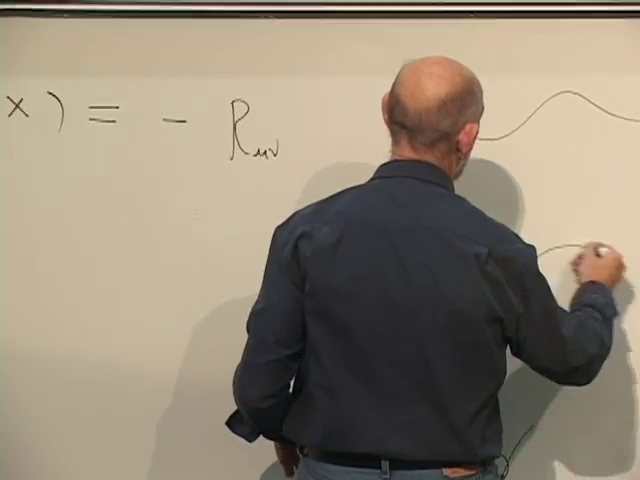
\includegraphics[width=0.76\textwidth]{lecture_09_figure_07.png}
  \caption{計量の変化は、リッチテンソルの負として模式的に書かれ、その横に平滑化曲線が描かれている。}
  \lectureframe{00:43:00}
  \label{fig:l09-ricci-flow-board}
\end{figure}

\begin{classroomqa}
\audiencequestion{振動子のカットオフ\(N\)は、この流れの方程式のどこに現れるのでしょうか。\lecturetimestamp{00:43:38}}
\lecturerresponse{それはスケール変数です。含まれる最高次のモードが変わると、弦の大きさの和は対数的に変化するので、自然な発展パラメータは\(\log N\)、あるいは同等に\(\log\Lambda\)です。式\eqref{eq:l09-ricci-flow}は、モードの1つの対数的な殻によって引き起こされる無限小の変化を記述しています。}
\end{classroomqa}

許容される背景とは、この流れの固定点です。主要な次数では、
\begin{equation}
  \boxed{R_{\mu\nu}=0.}
  \label{eq:l09-ricci-flat}
\end{equation}
リッチ平坦とは、リーマンテンソルのすべての成分が消えることを意味しません。たとえば重力波は、真空において\(R_{\mu\nu}=0\)を満たしながら、非零の曲率を持つことができます。

\subsection{同じ条件が真空アインシュタイン方程式である}

従来の定数を抑制すると、アインシュタイン方程式は
\begin{equation}
  G_{\mu\nu}
  \equiv
  R_{\mu\nu}-\frac12 g_{\mu\nu}R
  =T_{\mu\nu}.
  \label{eq:l09-einstein}
\end{equation}

\begin{figure}[H]
  \centering
  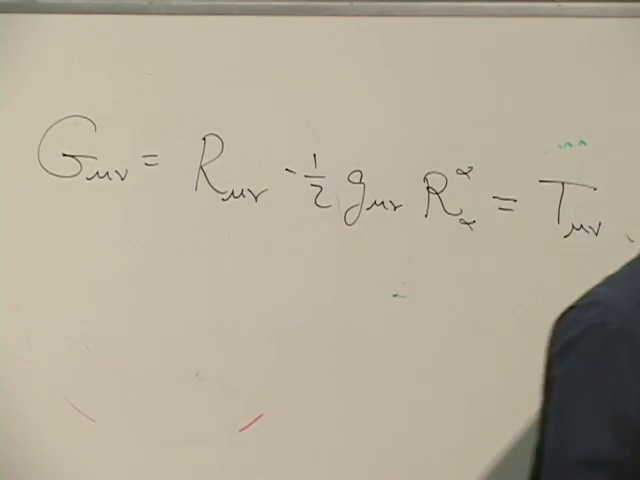
\includegraphics[width=0.78\textwidth]{lecture_09_figure_08.png}
  \caption{黒板上のアインシュタインテンソルと応力テンソル。}
  \lectureframe{00:47:15}
  \label{fig:l09-einstein-board}
\end{figure}

真空では\(T_{\mu\nu}=0\)。\(D\)時空次元でトレースを取ると
\begin{equation}
  0=g^{\mu\nu}G_{\mu\nu}
   =\left(1-\frac{D}{2}\right)R.
  \label{eq:l09-einstein-trace}
\end{equation}
\(D\neq2\)のとき、\(R=0\)であり、\eqref{eq:l09-einstein}に代入し直すと\(R_{\mu\nu}=0\)が得られます。したがって、弦がそのカットオフ依存性を失うという条件は、真空重力場の方程式です。重力は理論に付け加えられたのではなく、整合性の代償として現れたのです。

\emph{真空}という言葉は、何も起こらないという意味ではありません。それは、その領域に応力エネルギー源が存在しないという意味です。源のないマクスウェル方程式は電磁波を許容し、源のないアインシュタイン方程式は重力波を許容します。リッチテンソルが消えていても、幾何は動的であり得ます。

\begin{classroomqa}
\audiencequestion{この条件は共形不変性と関係があるのでしょうか。\lecturetimestamp{00:52:20}}
\lecturerresponse{はい、ただし質問は録音の中で一部失われています。関連する対称性は、\emph{世界面}量子理論の共形不変性です。世界面のスケール異常が消えることを要求することが、計量のベータ関数をゼロに設定するものです。これは、時空自体の共形不変性を要求することと混同されるべきではありません。}
\end{classroomqa}

第二の整合性条件があります。世界面の共形不変性は、臨界時空次元も固定します。超弦では10、ボソン弦では26です。したがって、リッチ平坦性だけが要件の完全なリストではありませんが、アインシュタイン方程式を最も直接的に示す部分です。

\section{欠けている次元ではなくコンパクトな次元}

超弦の背景は9つの空間次元と1つの時間次元を持ちます。我々の巨視的な世界は3つの大きな空間方向しか示さないので、6つの空間次元は隠されているか、通常のスケールではアクセスできないようにされていなければなりません。コンパクト化は、それらを真の方向として保ちながら、小さな有限の広がりを与えます。

\begin{classroomqa}
\audiencequestion{異なる観測者が異なる時計を持ち運ぶなら、それは1つ以上の時間次元を持つことに相当するのでしょうか。\lecturetimestamp{00:56:59}}
\lecturerresponse{いいえ。多くの時計とは、1つの時空における座標を測定する多くの計器であり、独立した時間的方向を生み出すものではありません。ここで考えられている余分な次元は空間的です。馴染み深い量子論的および因果的構成は、複数の局所的時間方向を持つ同様に整合的な理論を与えないので、その可能性はこのコンパクト化模型の一部ではありません。}
\end{classroomqa}

自分たちの世界が線であると信じている生き物を想像してください。低い解像度では、彼らは前後にしか動けません。しかし、十分に強力な顕微鏡の下では、その線は非常に細い円筒であることが明らかになります。小さな生き物は、その長さに沿ってだけでなく、円形の方向の周りも動くことができます。第二の方向は常に存在していましたが、その円周は粗い探査では分解できないほど小さかったのです。

\begin{figure}[H]
  \centering
  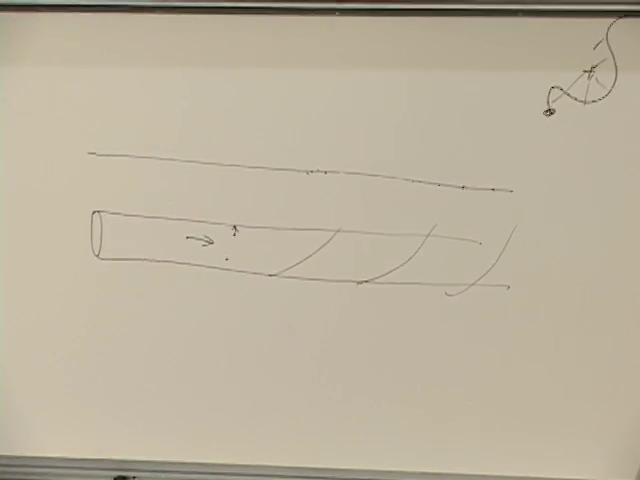
\includegraphics[width=0.78\textwidth]{lecture_09_figure_09.png}
  \caption{細い円筒と、その隠された円形方向を巻き回る軌道。}
  \lectureframe{01:01:00}
  \label{fig:l09-hidden-cylinder}
\end{figure}

円筒は、上端と下端が同一視された帯として表すことができます。上端を越えると、同じ縦方向の位置で下端を通って戻ります。どちらの端にも物理的な境界はありません。同じ操作を2つの方向で行うことができます。長方形の左端と右端を同一視し、さらにその上端と下端も同一視します。結果は2次元トーラスです。

\begin{figure}[H]
  \centering
  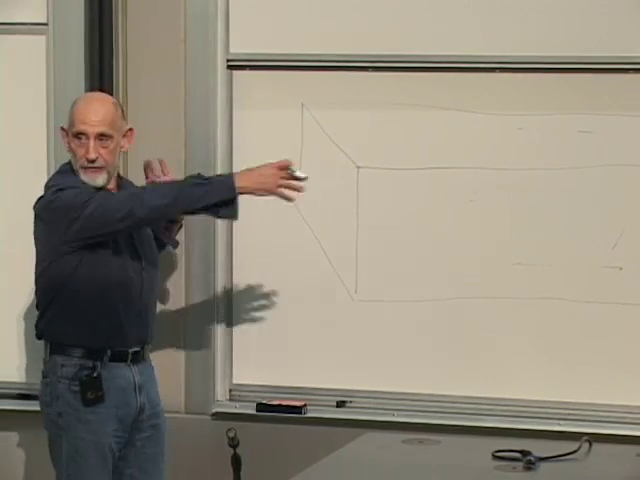
\includegraphics[width=0.76\textwidth]{lecture_09_figure_10.png}
  \medskip

  \begin{tikzpicture}[x=0.82cm,y=0.82cm,>=Latex]
    \draw[thick] (0,0) rectangle (4,2.15);
    \draw[blue!65!black,->] (0,2.48) -- (4,2.48);
    \draw[blue!65!black,->] (4,-0.34) -- (0,-0.34);
    \node at (2,-0.82) {one periodic direction};
    \draw[thick] (6.1,0) rectangle (10.1,2.15);
    \draw[blue!65!black,->] (6.1,2.48) -- (10.1,2.48);
    \draw[blue!65!black,->] (10.1,-0.34) -- (6.1,-0.34);
    \draw[red!70!black,->] (5.76,0) -- (5.76,2.15);
    \draw[red!70!black,->] (10.44,2.15) -- (10.44,0);
    \node at (8.1,-0.82) {two periodic directions};
  \end{tikzpicture}
  \caption{黒板のスラブと、きれいな基本領域の記述。1つの端の対を同一視すると円筒が得られ、両方の対を同一視するとトーラスが得られます。}
  \lectureframe{01:04:40}
  \label{fig:l09-periodic-identification}
\end{figure}

トーラスは、三次元空間におけるベーグル形の曲面である前に、まず位相である。トーラスを一度切断すると円筒になり、もう一度切断すると、辺の同一視を覚えておくならば、長方形になる。この長方形には平坦な計量を入れることができるので、得られる平坦トーラスは局所的にリーマン曲率がゼロであり、確かにリッチ平坦である。

長方形上の直線的軌道は、同一視された辺を越えてまっすぐに続く。その傾きが二つの周期の有理比であれば、軌道はやがて閉じる。比が無理数であれば、決して閉じず、トーラス上で稠密になる。

\begin{figure}[H]
  \centering
  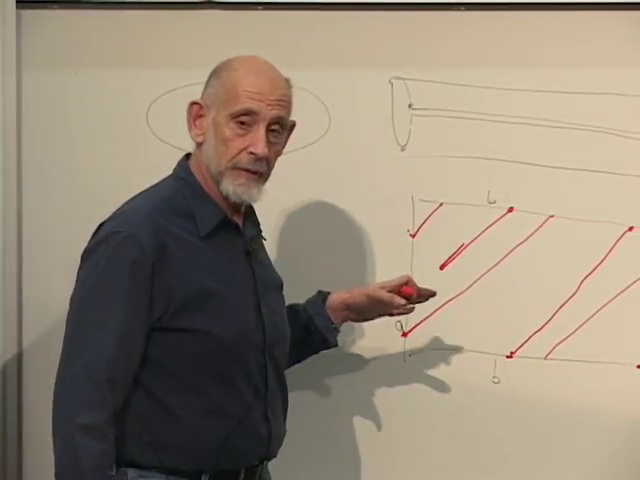
\includegraphics[width=0.76\textwidth]{lecture_09_figure_11.png}
  \caption{基本領域内の繰り返される直線部分は、トーラス上の一つの途切れない軌道を表す。}
  \lectureframe{01:11:00}
  \label{fig:l09-torus-trajectory}
\end{figure}

高次元トーラスも同じようにして作られる。各対の向かい合う面を同一視した立方体は三次元トーラスであり、六つのコンパクトな方向は六次元トーラスによってモデル化できる。これらの対象をすべて通常の三次元空間に埋め込もうとしてはいけない。面の同一視による記述は内在的であり、完全である。

\begin{classroomqa}
\audiencequestion{余分な次元は必ずそれ自身に戻ってこなければならないのだろうか。
\lecturetimestamp{01:15:03}}
\lecturerresponse{定理としてそうなるわけではない。非コンパクトでありえても、その場合には通常、観測される長距離の世界におけるもう一つの大きな方向として現れるであろう。コンパクト性は、余分な次元とその見かけ上の不在を両立させる最も単純な方法である。なぜ自然が特定のコンパクト化を選ぶのかは、別の力学的问题である。}
\end{classroomqa}

\begin{classroomqa}
\audiencequestion{なぜ、見えない次元がこのように丸め込まれた通常の空間的方向であり、まったく別の何かではないと仮定するのか。\lecturetimestamp{01:15:51}}
\lecturerresponse{これが明確で可解な仮説だからであり、自然の唯一の記述であると証明されたからではない。コンパクトな空間多様体は、整合的な例を構成し、そのスペクトルを計算することを可能にする。よりエキゾチックな可能性は、同じことを行うことによってその地位を獲得しなければならない。}
\end{classroomqa}

\begin{classroomqa}
\audiencequestion{よく知られたベーグル形のトーラス上の距離は、長方形における距離のようには見えない。どちらの幾何が意味されているのか。
\lecturetimestamp{01:18:11}}
\lecturerresponse{\emph{トーラス}という用語は同一視を固定するのであって、一つの一意な計量を固定するのではない。埋め込まれたベーグルは三次元空間から曲がった計量を受け継ぐ。周期的に同一視された長方形は平坦な計量を担う。それらは同じ位相を持ち、異なる幾何を持つ。単純なコンパクト化については平坦な方を意味している。}
\end{classroomqa}

\section{平坦トーラスの形状パラメータ}

平坦な二次元トーラスでさえ一意ではない。その基本平行四辺形は全体の面積、アスペクト比、ずれを持つ。これらのパラメータを変えると距離が変わり、したがって位相を変えることなくスペクトルが変わる。

\begin{figure}[H]
  \centering
  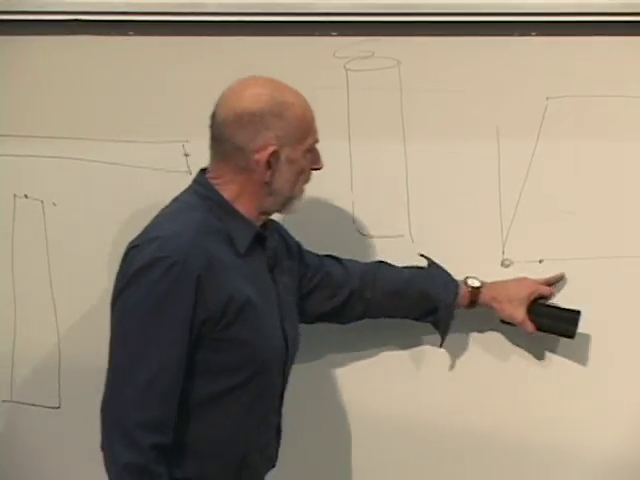
\includegraphics[width=0.74\textwidth]{lecture_09_figure_12.png}
  \medskip

  \begin{tikzpicture}[x=0.9cm,y=0.9cm,>=Latex]
    \draw[thick] (0,0) rectangle (3.4,2.1);
    \draw[<->] (0,-0.35) -- node[below] {\(L_1\)} (3.4,-0.35);
    \draw[<->] (-0.35,0) -- node[left] {\(L_2\)} (-0.35,2.1);
    \draw[thick] (5.4,0) -- (8.8,0) -- (9.7,2.1) -- (6.3,2.1) -- cycle;
    \draw[dashed] (5.4,0) -- (6.3,2.1);
    \draw[->] (5.75,2.48) -- node[above] {shear} (6.45,2.48);
    \node at (1.7,-1.00) {area and aspect ratio};
    \node at (7.55,-1.00) {complex structure};
  \end{tikzpicture}
  \caption{トーラスのモジュライを議論するために用いられる長方形およびずらされた基本領域。}
  \lectureframe{01:23:00}
  \label{fig:l09-torus-moduli}
\end{figure}

二次元トーラスについては、形状を複素数\(\tau=\tau_1+i\tau_2\)にまとめると便利である。実部はずれを記録し、虚部は全体のスケールを分離した後のアスペクト比を記録する。二つの基本サイクルを入れ替えたり、それらの整数基底を変えたりすると、見かけ上異なる平行四辺形が同じトーラスを記述することがある。

\begin{classroomqa}
\audiencequestion{同一視の前に一方の辺を反転させるとどうなるか。\lecturetimestamp{01:24:20}}
\lecturerresponse{それは異なる位相を生じる。反射を伴う同一視は、通常のトーラスではなく、非orientableな曲面であるクラインの壺を与える。}
\end{classroomqa}

\begin{classroomqa}
\audiencequestion{ねじれが辺に沿って一様でない場合はどうか。
\lecturetimestamp{01:25:01}}
\lecturerresponse{滑らかな非一様変形は、基本領域上の計量に移すことができる。位相的同一視と幾何学的データは区別して保たなければならない。貼り合わせを変えると位相が変わりうるが、距離を滑らかに変えると計量が変わる。}
\end{classroomqa}

\editorialnote{平坦な二次元トーラスについて、面積は最も単純なケーラー・モジュラスであり、\(\tau\)は複素構造モジュラスである。連続的なずれは\(\tau\)の一部である。一方、デーン・ツイストは離散的な写像類群の操作であり、\(\tau\mapsto\tau+1\)で表される。それ自体は連続的モジュラスではない。これは、板書での議論中に用いられた意図的に非形式的な用語を明確にするものである。}

平坦トーラスは整合性条件を直ちに満たすため有用であるが、その対称性は素粒子物理学の現実的モデルにはあまりに寛大すぎる。より入り組んだリッチ平坦空間、特にカラビ--ヤウ多様体は、より豊かなコンパクト化を与える。その詳細な構成はこの議論の範囲を超えるが、原理は同じままである。

\section{コンパクト円をそのスペクトルから読み取る}

休憩の後、コンパクト空間を周長\(2\pi R\)の1つの円に縮約する。波動関数は一周した後で一価でなければならない：
\begin{equation}
  e^{ip_c(x+2\pi R)/\hbar}=e^{ip_cx/\hbar}.
\end{equation}
したがって
\begin{equation}
  p_cR=n\hbar,
  \qquad
  p_c=\frac{n\hbar}{R},
  \qquad n\in\mathbb Z.
  \label{eq:l09-kk-momentum}
\end{equation}

\begin{figure}[H]
  \centering
  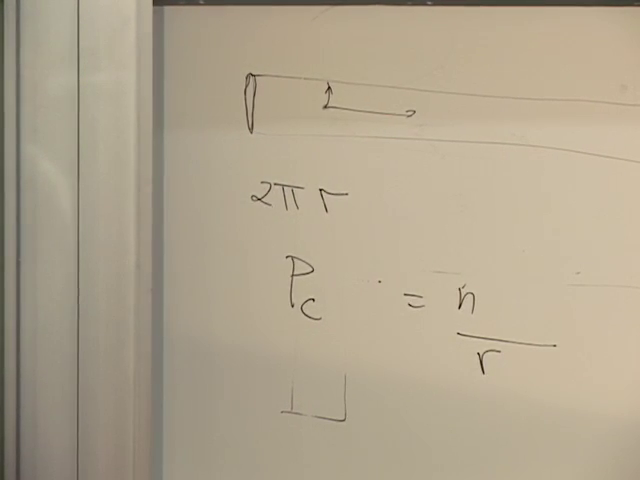
\includegraphics[width=0.74\textwidth]{lecture_09_figure_13.png}
  \caption{コンパクトな周長\(2\pi R\)と量子化された運動量
  \(p_c=n\hbar/R\)。}
  \lectureframe{01:32:15}
  \label{fig:l09-kk-board}
\end{figure}

全時空における質量のない粒子に対して、
\begin{equation}
  E=c|\mathbf P|.
  \label{eq:l09-massless-dispersion}
\end{equation}

\begin{figure}[H]
  \centering
  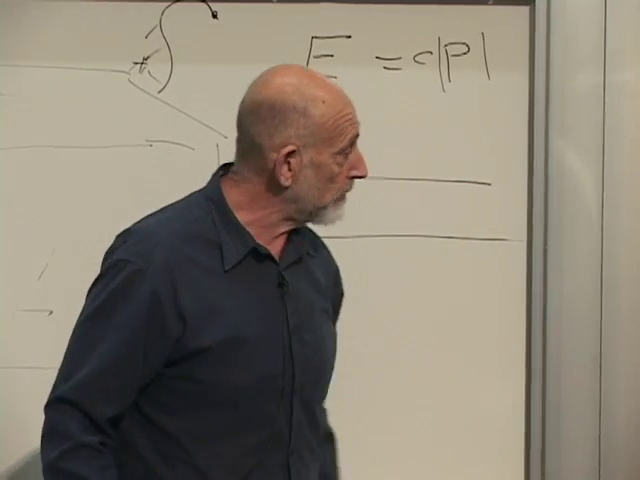
\includegraphics[width=0.70\textwidth]{lecture_09_figure_14.png}
  \caption{コンパクトな運動量を低次元の質量として再解釈するために用いられる質量のない分散関係。}
  \lectureframe{01:33:45}
  \label{fig:l09-massless-board}
\end{figure}

運動量を非コンパクト部分とコンパクト部分に分け、
\(c=\hbar=1\)と置く：
\begin{equation}
  E^2=\mathbf p_{\mathrm{large}}^2+\frac{n^2}{R^2}.
  \label{eq:l09-kk-dispersion}
\end{equation}
コンパクト方向を分解できない観測者は、これを
\(E^2=\mathbf p_{\mathrm{large}}^2+m^2\)と比較し、質量の塔
\begin{equation}
  m_n=\frac{|n|}{R}.
  \label{eq:l09-kk-masses}
\end{equation}を推論する。
\(n\)の2つの符号は、正と負の質量ではなく、同じ正のエネルギーをもつ反対向きのコンパクト運動量を表す。したがって間隔\(1/R\)は半径を分光学的に明らかにする。これがKaluza--Klein機構である：隠れた方向の運動量が、可視の次元における質量として現れる。

\section{巻き付き状態がスペクトルを完成させる}

閉じた弦には、点粒子には不可能な可能性がある：円の周りに巻き付くことができる。巻き付き数が\(w\)ならば、弦はコンパクト方向を\(w\)回覆って初めて閉じる。その長さは\(2\pi |w|R\)なので、張力がエネルギー
\begin{equation}
  m_w
  =2\pi T\,|w|R
  =\frac{|w|R}{\alpha'}.
  \label{eq:l09-winding-mass}
\end{equation}を与える。
講義では\(\alpha'=1\)の単位を選び、これを
\begin{equation}
  m_w=|w|R.
  \label{eq:l09-winding-lecture-units}
\end{equation}に簡約する。
正と負の\(w\)は、円の周りの反対向きの配向である。

\begin{figure}[H]
  \centering
  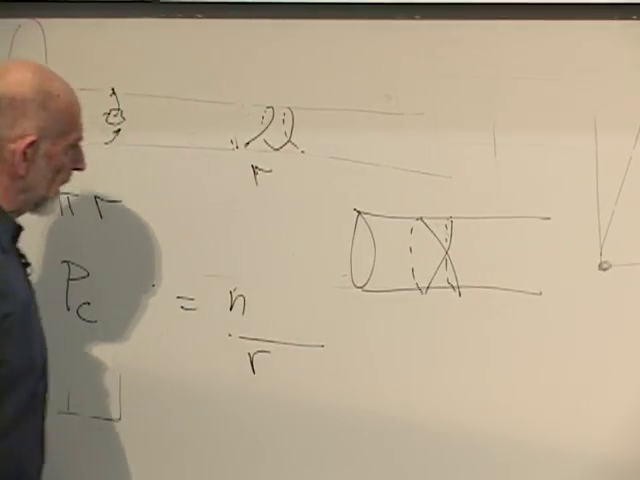
\includegraphics[width=0.76\textwidth]{lecture_09_figure_15.png}
  \caption{コンパクトな円筒に巻き付いた閉じた弦。コンパクト半径が黒板に記されている。}
  \lectureframe{01:39:45}
  \label{fig:l09-winding-board}
\end{figure}

したがってコンパクト円は2つの相補的な梯子を生み出す：
\begin{equation}
  m_n=\frac{|n|}{R},
  \qquad
  m_w=\frac{|w|R}{\alpha'}.
  \label{eq:l09-two-towers}
\end{equation}
\(R\)が大きいとき、運動量準位は互いに近く、巻き付き状態は重い。\(R\)が小さいとき、運動量準位は互いに遠く、巻き付き状態は軽い。

\begin{figure}[H]
  \centering
  \begin{tikzpicture}[x=1cm,y=0.9cm,>=Latex]
    \draw[->] (0,0) -- (0,4.7) node[above] {\(m\)};
    \foreach \y/\lab in {0/0,1.1/{1/R},2.2/{2/R},3.3/{3/R},4.4/{4/R}} {
      \draw (-0.16,\y) -- (0.16,\y);
      \node[left] at (-0.22,\y) {\(\lab\)};
    }
    \node at (0,-0.62) {momentum};
    \draw[<->,very thick,blue!65!black] (2.05,2.15) -- (4.05,2.15)
      node[midway,above] {\(R\leftrightarrow\alpha'/R\)};
    \draw[->] (6.1,0) -- (6.1,4.7) node[above] {\(m\)};
    \foreach \y/\lab in {0/0,1.1/{R/\alpha'},2.2/{2R/\alpha'},3.3/{3R/\alpha'},4.4/{4R/\alpha'}} {
      \draw (5.94,\y) -- (6.26,\y);
      \node[right] at (6.32,\y) {\(\lab\)};
    }
    \node at (6.1,-0.62) {winding};
  \end{tikzpicture}
  \caption{半径が弦単位で反転されると、運動量の塔と巻き付きの塔が入れ替わる。}
  \label{fig:l09-dual-mass-towers}
\end{figure}

\section{T双対性：小さい円と大きい円は同じ物理である}

2つの塔は
\begin{equation}
  R\longleftrightarrow\frac{\alpha'}{R},
  \qquad
  n\longleftrightarrow w.
  \label{eq:l09-t-duality}
\end{equation}によって入れ替わる。
黒板で用いられている単位では\(\alpha'=1\)なので、これは単に
\(R\leftrightarrow1/R\)である。自己双対半径
\(R=\sqrt{\alpha'}\)では、運動量と巻き付きのスケールが一致する。

\begin{figure}[H]
  \centering
  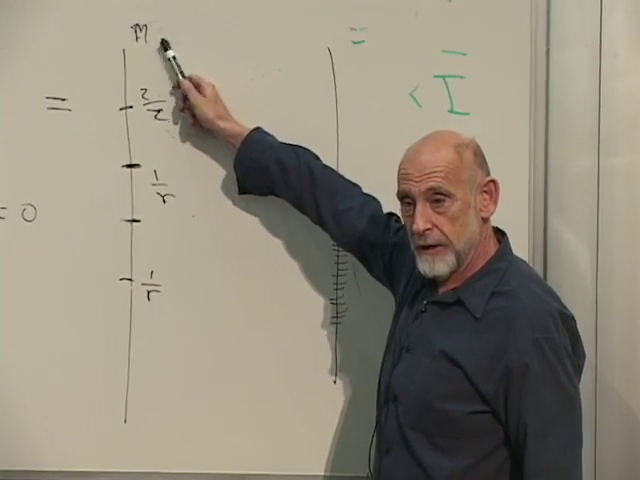
\includegraphics[width=0.74\textwidth]{lecture_09_figure_16.png}
  \caption{半径が自己双対スケールを横切るとき、黒板で比較された疎な質量梯子と密な質量梯子。}
  \lectureframe{01:43:00}
  \label{fig:l09-duality-board}
\end{figure}

初等的な質量公式の入れ替えは、この結果の目に見える端にすぎない。閉じた弦の振動子状態と散乱振幅もまた整合的に写像される。弦スケールより小さい円は、ますます微小になる新しい幾何ではなく、より大きい双対円として等価な記述をもつ。点粒子は運動量モードをもつが巻き付きモードをもたないため、この同一視を行うことができない。

\begin{classroomqa}
\audiencequestion{これは単に縦方向と横方向を入れ替えるのと同じことか？\lecturetimestamp{01:44:38}}
\lecturerresponse{いいえ。これは2つの異なる量子数を入れ替える：円の周りの運動量と、閉じた弦が円を巻き付く回数である。同時に半径を反転しなければならない。}
\end{classroomqa}

\begin{classroomqa}
\audiencequestion{\(R<\sqrt{\alpha'}\)と
\(R>\sqrt{\alpha'}\)における記述はボソンだけを指すのか、それともフェルミオンも指すのか？
\lecturetimestamp{01:46:30}}
\lecturerresponse{この双対性は、それを明らかにするために用いられた単純なボソン的質量梯子だけでなく、完全なコンパクト化された弦理論の対称性である。セクターの詳細な写像は理論に依存するが、小--大の等価性は1つの粒子種に限られない。}
\end{classroomqa}

\begin{classroomqa}
\audiencequestion{比較されている2つの状態は開いた弦か、それとも閉じた弦か？\lecturetimestamp{01:47:32}}
\lecturerresponse{それらは閉じた弦の状態である。自由に伝播する閉じた弦はコンパクト円に巻き付くことができる。自由な端点をもつ通常の開いた弦は、同じ保存された巻き付き数をもたない。}
\end{classroomqa}
\editorialnote{より完全な開いた弦の説明では、T双対性はNeumann境界条件とDirichlet境界条件を入れ替え、Dブレーンを導入する。だからこそ開いた弦のT双対性は、閉じた弦の巻き付き公式を単に写すよりも豊かなのである。}

\begin{classroomqa}
\audiencequestion{この入れ替えは、ブラックホールの事象の地平面近傍における空間と時間の交換に類似しているのか。\lecturetimestamp{01:48:00}}
\lecturerresponse{いいえ。地平面座標と因果的な性格は別の問題である。ここでは二つの記述は一つのコンパクトな空間的円周に関わり、その運動量セクターと巻き付きセクターの交換を扱っている。}
\end{classroomqa}

\begin{classroomqa}
\audiencequestion{これは最小長さを与えることで短距離の自己エネルギーの問題を解決するのか。\lecturetimestamp{01:48:35}}
\lecturerresponse{弦のスケールより小さい半径は新たな不等価な円背景を定義しないことを示している。\(R\)を自己双対点を超えて減少させると、双対半径が増加する。これは任意に小さい円の幾何を探ることを妨げる厳密な弦理論的障害であるが、考え得るあらゆる距離の概念が一つの普遍的な固い下限を持つという主張に変えてはならない。}
\end{classroomqa}

\section{巻き付きセクターを省略できない理由}

\begin{classroomqa}
\audiencequestion{巻き付いていない弦のみを用いて理論を定義し、巻き付き状態を除外することはできるか。\lecturetimestamp{01:48:56}}
\lecturerresponse{いいえ。閉弦の相互作用がそれらを生成する。巻き付いていないループをコンパクト方向の周りに引き伸ばし、一方の線分が円周を一方向にたどり、別の線分が反対方向にたどるようにする。正味の巻き付き数は依然としてゼロである。その後、再接続によってループは巻き付き数\(+1\)と\(-1\)を持つ二つの閉弦に分裂し得る。この対は離れ得るので、初期状態に巻き付き状態がなかったとしても、巻き付き状態はスペクトルに属さなければならない。}
\end{classroomqa}

\begin{figure}[H]
  \centering
  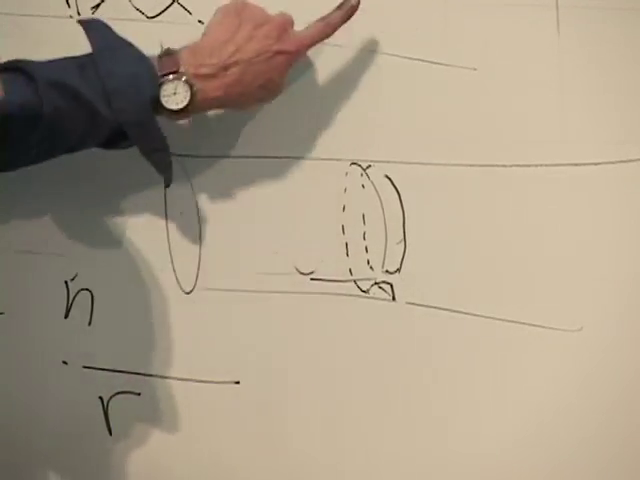
\includegraphics[width=0.74\textwidth]{lecture_09_figure_17.png}
  \caption{再接続前にコンパクト方向の周りに配置された、引き伸ばされた巻き付き数ゼロのループ。}
  \lectureframe{01:50:30}
  \label{fig:l09-winding-pair-before}
\end{figure}

\begin{figure}[H]
  \centering
  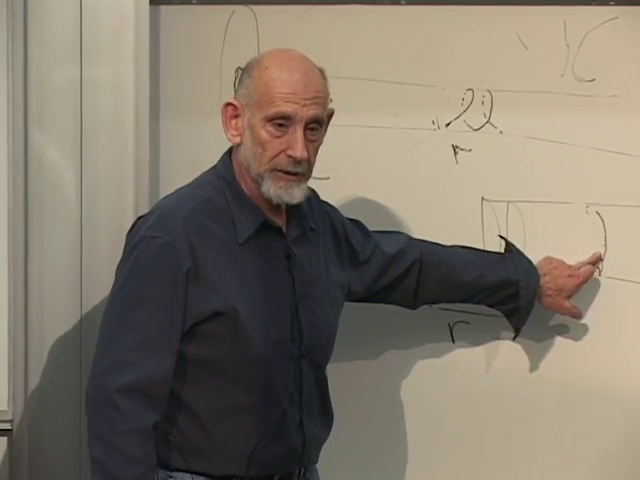
\includegraphics[width=0.72\textwidth]{lecture_09_figure_18.png}
  \medskip

  \begin{tikzpicture}[x=0.9cm,y=0.9cm,>=Latex]
    \draw[thick] (0,0) ellipse (1.0 and 1.55);
    \draw[blue!65!black,thick]
      (0.08,1.35) .. controls (2.0,1.15) and (2.0,-1.15) .. (0.08,-1.35);
    \draw[red!70!black,thick]
      (-0.08,-1.35) .. controls (-2.0,-1.15) and (-2.0,1.15) .. (-0.08,1.35);
    \node at (0,-2.15) {net \(w=0\)};
    \draw[->,thick] (2.45,0) -- (3.75,0) node[midway,above] {split};
    \draw[thick] (5.05,0.62) ellipse (0.68 and 1.02);
    \draw[blue!65!black,very thick,->]
      (5.05,1.64) arc[start angle=90,end angle=-250,x radius=0.68,y radius=1.02];
    \node at (5.05,-0.82) {\(w=+1\)};
    \draw[thick] (7.45,0.62) ellipse (0.68 and 1.02);
    \draw[red!70!black,very thick,<-]
      (7.45,1.64) arc[start angle=90,end angle=-250,x radius=0.68,y radius=1.02];
    \node at (7.45,-0.82) {\(w=-1\)};
  \end{tikzpicture}
  \caption{黒板に示された分離した巻き付きループと、巻き付き--反巻き付き対生成の明快な再構成。全巻き付き数はゼロのままである。}
  \lectureframe{01:51:30}
  \label{fig:l09-winding-pair-after}
\end{figure}

\begin{classroomqa}
\audiencequestion{巻き付き対を生成するには余分なエネルギーが必要か。
\lecturetimestamp{01:52:11}}
\lecturerresponse{はい。弦を引き伸ばすには張力エネルギーがかかり、最終的な巻き付いた弦は\eqref{eq:l09-winding-mass}にある質量を持つ。十分に高エネルギーの衝突はこの対を生成し得る。ちょうど、衝突が関連する保存電荷を保ちながら粒子とその反粒子を生成し得るのと同じである。}
\end{classroomqa}

\section{弦の背景の形を聴き取ることはできるか。}

通常のコンパクト化された粒子理論では、カルツァ--クライン・スペクトルの間隔から半径を推測できる。すなわち、その固有振動モードからコンパクト空間の形を聴き取ろうとするのである。弦理論はこの逆問題をより微妙なものにする。運動量モードは\(1/R\)を聴き取り、巻き付きモードは\(R/\alpha'\)を聴き取り、二つを交換しても完全なスペクトルは変わらない。点粒子の幾何が異なると見なす二つの半径は、双対変数で記述された一つの弦背景である。

したがって講義は、約束された二つの結論の双方に一つの道筋で到達した。紫外完全性は標的計量が真空アインシュタイン方程式を満たすことを強制するので、重力は不可避である。次にコンパクト化は隠れた幾何を粒子スペクトルに変えるが、巻き付き状態はそのスペクトルが弦のスケールより下で一意な古典的半径を割り当てることを妨げる。整合性はどの幾何が許されるかを選ぶだけでなく、T双対性を通じて、何がそもそも別個の幾何として数えられるかを変えるのである。
